\documentclass{article}
\usepackage{graphicx} 
\usepackage{amsmath}
\bibliographystyle{plain} 
\usepackage{hyperref}
\usepackage{qcircuit}
\hypersetup{
     colorlinks   = true,
     linkcolor    = blue,
     citecolor    = blue
}


\title{CHSH on Bell’s inequalities and how we could use them to send information over distances.}
\author{Adam Jurkowski, Mark Agib, Seaena Kim}
\date{July 2025}

\begin{document}
\maketitle

\begin{abstract}
    Entanglement is the cornerstone of quantum computation and is essential in quantum algorithms. Generating long-range and high-quality entanglement is a necessary milestone for current hardware to reach. We attempt to quantify the quality of entanglement on a quantum computer for distant qubits using Clauser-Horne-Shimony-Holt (CHSH) inequality violations. This is done through simulations on a full circuit noise model using distances ranging from 2 to 12.
\end{abstract}



\section{Introduction}
Until the mid-1900s, the principle of locality, stating that objects are solely influenced by their immediate surroundings, remained unquestioned. In 1935, Einstein, Podolsky, and Rosen established the EPR paradox, which exposed quantum mechanics’ violation of the principle of locality, opening up theories of local hidden variables \cite{PhysRev.47.777}. The paradox suggested that current quantum theory implied nonlocal effects, which he famously called "spooky action at a distance." In order to resolve this problem, EPR proposed the idea of local hidden variables that would preserve locality and determinism. However, EPR was challenged by John Stweart, who introduced mathematical inequalities, and it offered an experimental violation that would rule out EPR's theory of hidden variables and confirm the presence of non-local quantum correlations \cite{PhysicsPhysiqueFizika.1.195}. Subsequent experiments, like that of Clauser-Horne-Shimony-Holt (CHSH) formulation of Bell's theorem, provided increasing support of quantum mechanics and laid the foundation for understanding quantum entanglement. 

This paper aims to investigate the CHSH version of Bell's inequalities to quantify the quality of entanglement between distant qubits on quantum processors. Entanglement is essential for any application of quantum computing, such as quantum teleportation, quantum key distribution, quantum algorithms, and more. As such, ensuring that Noisy Intermediate Scale Quantum (NISQ) devices can successfully create high-quality entanglement is necessary for the success of the field. 

\section{Literature Review}

John Clauser and Stuart Freedman were the first to test Bell’s inequalities in 1972. A researcher at UC Berkeley, Clauser, explored entangled photons with graduate student Freedman \cite{PhysRevLett.28.938}. Before the experiment, Clauser and his colleagues, Michael Horne, Abner Shimony, and Richard Holt, created the CHSH inequality, a variant of Bell’s theorem, as a way to experimentally test Bell’s original inequality \cite{PhysRevLett.23.880}. The CHSH inequality is as follows:

\begin{equation} \label{eq1}
\begin{split}
    S & \leq 2
\end{split}
\end{equation}
such that 
\begin{equation} \label{eq2}
\begin{split}
    S & = E(A,B) - E(A, B') +E(A', B) + E(A', B')
\end{split}
\end{equation}

Suppose $A$ and $B$ are Alice and Bob at opposite ends of a certain distance. Alice and Bob each have their two observables $(a, a’)$ and $(b, b’)$ that measure qubits. 4 distinct combinations are possible from the 4 measurements. Each term, such as $E(a,b)$, represents the quantum correlations of the four pairs, where $E()$ calculates the average of the products of the pairs over multiple runs. If the value $S$ is either less than $-2$ or greater than $2$, the particles are in entangled states and do not behave under theories of locality or hidden variables. 

There are four crucial elements of understanding quantum circuits and mechanics: Entanglement, Superposition, Interference, and Measurement. Entanglement is what Bell's equation and CHSH focus on the most, where two or more qubits become intertwined with each other and are able to exchange information instantaneously. Superposition is when a qubit is in two or more states, positions, or phases at once. For instance, a coin can be both heads and tails until physically measured. Interference occurs when qubits add or subtract, meaning their wave-like behavior causes qubits to augment or cancel each other out. Measurement takes away the quantum behavior of a qubit to cater to how people can see them. Therefore, measuring causes qubits in superposition, like the plus state, to collapse into one state, either 1 or 0. These quantum fields are hard to explore even today due to environmental noise and the delicacy of quantum entanglement and superposition circuits. 

In Clauser and Freedman’s experiment, they utilized polarized photons from calcium atoms instead of Bell’s original intended electrons. These particles, called $\gamma_1$and $\gamma_2$, were measured $10$ feet apart and viewed by optical systems made up of two lenses, a wavelength filter, a removable and rotatable polarizer, and a single-photon detector. The following diagram depicts the system that Clauser and Freedman used: 

\begin{figure}
    \centering
    \includegraphics[width=1.0\textwidth]{figs/pic1.png}
    \caption{}
    \label{fig:system-diagram}
\end{figure}

The two detectors recorded two variables: coincidence rate of two-photon detection $[R(\varphi)]$ and the angle of the planes of linear polarization $[\varphi]$. If these particles behaved according to quantum mechanics, its behavior would invalidate local hidden-variable theory and reject Bell’s inequality which assumes the following: The two photons propagate as separate localized particles; A binary selection process occurs for each photon at each polarizer; All photons incident on a detector have a probability of detection that is independent of whether or not the photon has passed through a polarizer. Mathematically, these assumptions create the following inequalities:

$$-1 \leq \Delta(\varphi) \leq 0$$
where
$$\Delta(\varphi) = \frac{3R(\varphi)}{R_0} - \frac{R(3\varphi)}{R_0} - \frac{R_1+R_2}{R_0}$$

The following graph shows the quantum correlation between the coincidence rate defined by the angle of the polarizers, divided by the rate with both polarizers removed, and the angle. 

\begin{figure}
    \centering
    \includegraphics[width=1.0\textwidth]{figs/pic2.png}
    \caption{}
    \label{fig:angles-graph}
\end{figure}

Using the CHSH Bell inequality and quantum mechanics, Clauser and Freedman were able to conclude that the behavior of these particles, measured by polarizer efficiencies and angles, rejected local hidden variable theories and upheld principles of entanglement. 
Since Clauser and Freedman’s experiment, scientists have used Bell’s inequalities to further back up quantum physics and theories. These experiments are performed to explore the utility of quantum behaving particles and potentially finding a way to send information over these qubits. In our experiment, we will utilize a quantum circuit and Bell’s inequality to find a way to efficiently send information over a certain distance without being intercepted by noise or other environmental factors. 


% lit rev2 
In Bartkiewicz, Horst, Lemr, and Miranowicz’s experiment, they explored extremal states of quantum mechanics. While the CHSH inequality is useful for testing the quantum behavior of some particles, there are extremes where particles can be entangled, but still abide by the CHSH inequality. Similar to the EPR paradox, particles can follow classical-leaning theorems, while having quantum characteristics such as entanglement. 
In the research paper Entanglement estimation from Bell inequality violation, scientists Bartkiewicz, Horst, Lemr, and Miranowicz used the CHSH inequality to explore states of 
particles that have quantum characteristics but do not violate the inequality. These states are known as Werner states and are applied to the following equation: 

$$\rho_W = p|\Psi^-\rangle \langle\Psi^-| + \frac{1 - p}{4}I \otimes I$$

where $|\Psi^-\rangle$ is the bell state $|\Psi^-\rangle = \frac{1}{\sqrt{2}} (|01\rangle - |10\rangle)$ and $p \in [0,1]$. 
 The CHSH inequality is violated when 
$\frac{1}{\sqrt{2}} < p \leq 1$
The particles are entangled when 
$\frac{1}{3} < p \leq 1$.
Therefore, while $\frac{1}{3} < p \leq \frac{1}{\sqrt{2}}$, the states are entangled and satisfy the CHSH inequality. 
The Karush-Kuhn-Tucker conditions, otherwise known as the saddle-point theorem, are applied to nonlinear programming in order to utilize the constrained optimization problem with inequalities. The four scientists used the KKT conditions as well as Lagrange multipliers which find the maximum and minimum values of a function (extremal states). From here, they explored the different concurrences of specific classes of qubits of two-qubit states. Using Monte Carlo simulations and the Horodecki measure, Bartkiewicz, Horst, Lemr, and Miranowicz were able to experiment with the boundaries of Bell’s inequality and entanglement. 
From this paper, we learned to acknowledge the limitations of the CHSH inequality while collecting our qubit circuit data. 

\subsection{CHSH for Quantum Computation}

Violation of the CHSH inequality has become a popular approach to measure entanglement on various types of quantum computers (quantum dot \cite{steinacker2025bell}, superconducting \cite{storz2023loophole}) and different types of matter. The first experimental validation of the Bell-CHSH inequality on a major quantum computer was done on IBM’s $5$ qubit computer in 2016. Many years later, the inequality still serves as one of the first measures of entanglement for any new quantum computer as proof of quantum mechanical properties. Besides the CHSH inequality, the three most common entanglement measures are negativity \cite{PhysRevA.65.032314}, concurrence \cite{PhysRevLett.80.2245}, and Relative Entropy of Entanglement (REE) \cite{PhysRevLett.78.2275}.


% Incomplete
Most recently, a short study conducted in 2025 used CHSH violations to explore the success of different CNOT implementations across distant qubits on \verb|ibm_qubec| \cite{waring2025chshviolationsusingdynamic}. As the distance between the entangled qubits rose, the CHSH Parameter (S) fell as expected. They found that the "post-processing" method of generating a CNOT gave the most success, and higher fidelity readout measurements would be necessary to achieve better results.

\section{Method}

We used the library \verb|Qiskit|’s AerSimulator \cite{qiskit2024} to simulate the created circuits using noise models from real IBM Quantum backends. Before the circuits are simulated, they need to be “transpiled”, which means translated to fit the topology of the specific device and for optimization on the specific hardware. For our case when \verb|optimization_level=3|, which is the highest level of optimization and finally we mapped the qubits to be neighboring each other. 

\begin{figure}
    \centering
    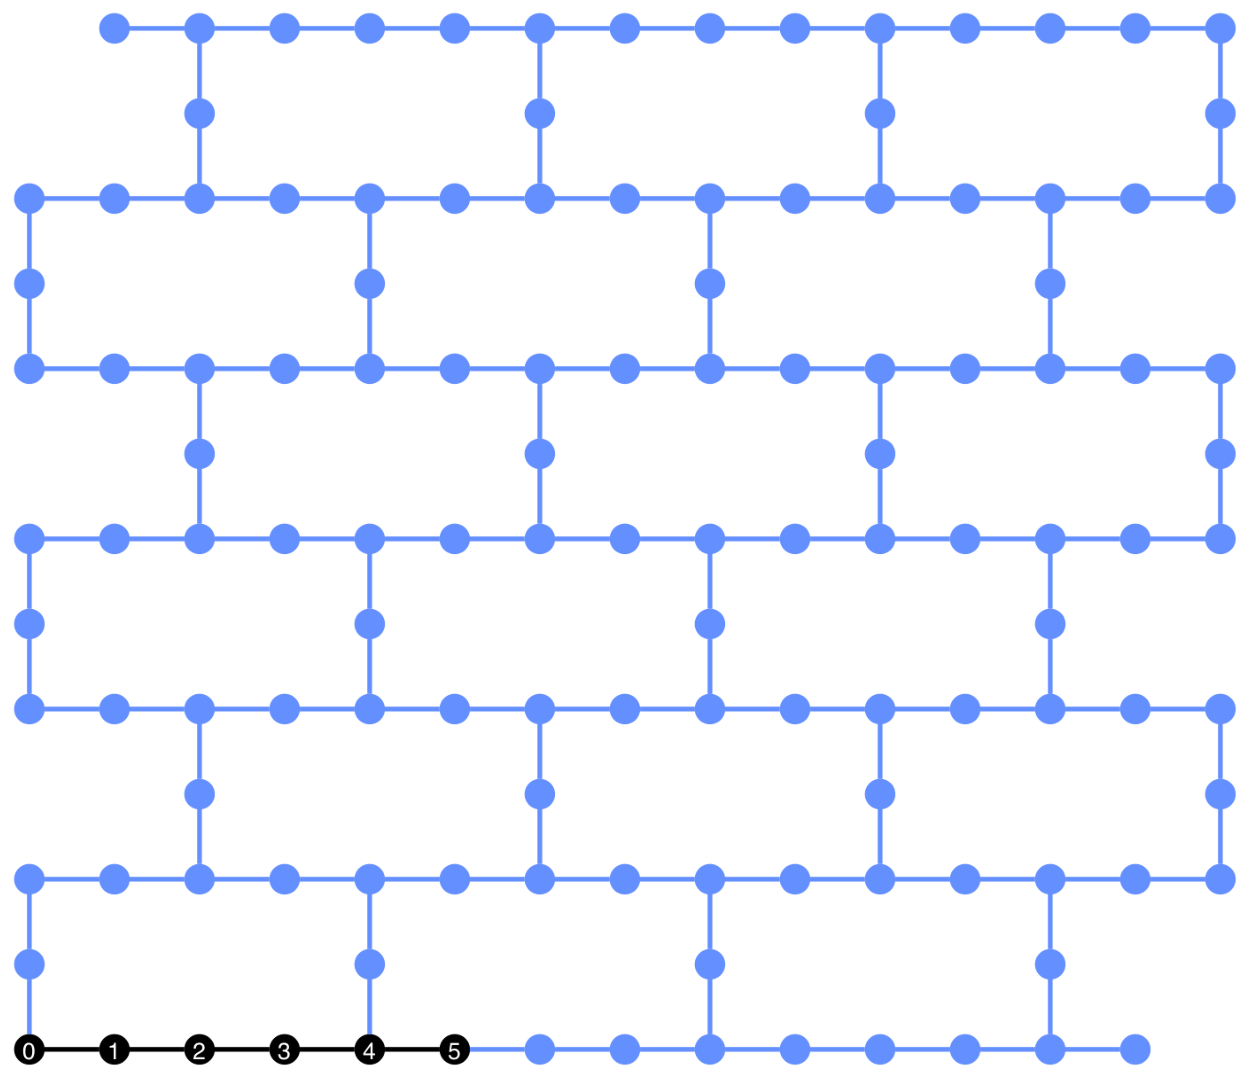
\includegraphics[width=1.0\textwidth]{figs/coupling_map.png}
    \caption{The coupling map of IBM brisbane's  $127$ qubits on the Eagle r3 processor is shown above. In the bottom left are the $6$ qubits used in a sample CHSH circuit.}
    \label{fig:coupling-map}
\end{figure}


\begin{figure}
    \centering
    \scalebox{1.25}{
        \[
            \Qcircuit @C=1em @R=1em {
            \lstick{\left| 0 \right\rangle} & \gate{H}  & \ctrl{1} \barrier[0em]{1} & \qw & \gate{H}  \barrier[0em]{1} & \qw & \meter  \\
            \lstick{\left| 0 \right\rangle} & \qw & \targ & \qw & \gate{R_y(\phi)} & \qw  &  \qw & \meter \\
            & \cw & \cw & \cw & \cw & \cw & \cw \cwx[-2] & \cw \cwx[-1] & \cw \\
            }
        \] 
    }
    \caption{An example circuit that would violate the CHSH inequality, where the top qubit is "Alice's" and the lower is "Bob's" qubit. We always begin with initializing the bell state (shown in the first section) and follow with a change of measurement basis based on the inputs. In the circuit shown above, Alice and Bob have received $x = 1$ and $y = 1$, respectively, creating their appropriate measurement bases. }
    \label{fig:circuit-basic}
\end{figure}

For the construction of our circuits, we began by creating a Bell state between the two qubits that would be Alice's and Bob’s, and then we applied different gates (based on the inputs) to change the measurement basis. When Alice was given a $0$, she would measure on a regular $Z$ basis, and given a $1$, she would measure on an $X$ basis (hence we apply a Hadamard). Traditionally the CHSH parameter’s value is maximized when Bob’ measures in the $\frac{Z+X}{\sqrt2}$ basis when given $0$ and $\frac{Z-X}{\sqrt2}$ basis when given $1$, which translates to $\frac{\pi}{4}$ rotations in the y-axis. 

In our case we tested 43 different phases between $\frac{\pi}{2}$ to $3\pi$. We chose 43 phases because it was the only number of phases between 31 and 100 that equally spaced intervals would include the optimal phase $\frac{\pi}{4}$. We also test on three different noise models (using \verb|NoiseModel.from_backend(backend)|) for the three backends: \verb|ibm_brisbane|, \verb|ibm_torino|, and \verb|ibm_sherbrooke|, which all have a heavy hex topology. The only difference is the processor, \verb|ibm_torino| has the Heron R1, and the rest have the Eagle R3. For each noise model, we try distances from $2$ qubits (standard circuit) to $12$ qubits.

\section{Findings}



\begin{figure}
    \centering
    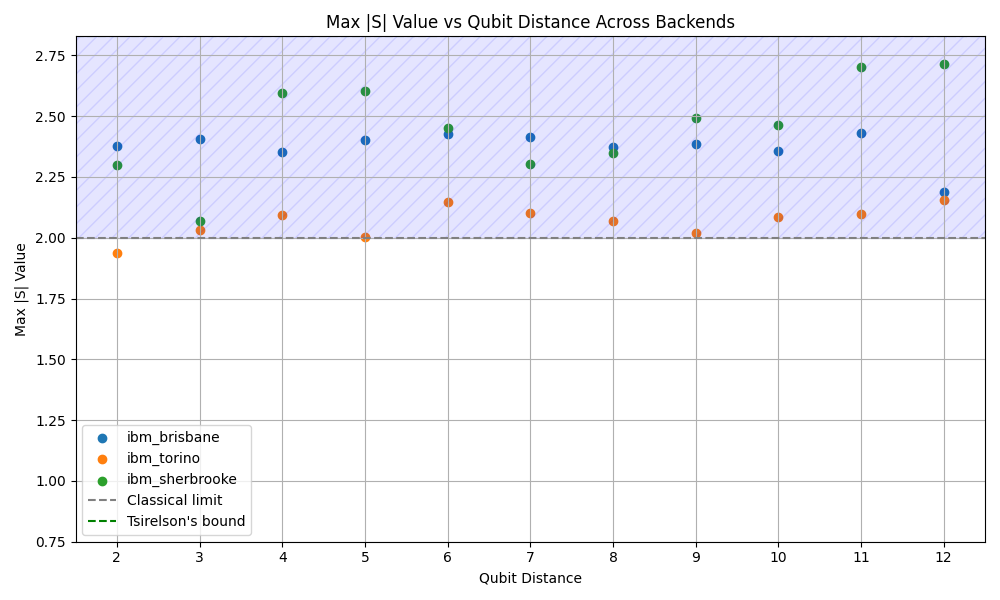
\includegraphics[width=1.0\textwidth]{figs/max vs qubit distance.png}
    \caption{}
    \label{fig:all}
\end{figure}

\begin{figure}
    \centering
    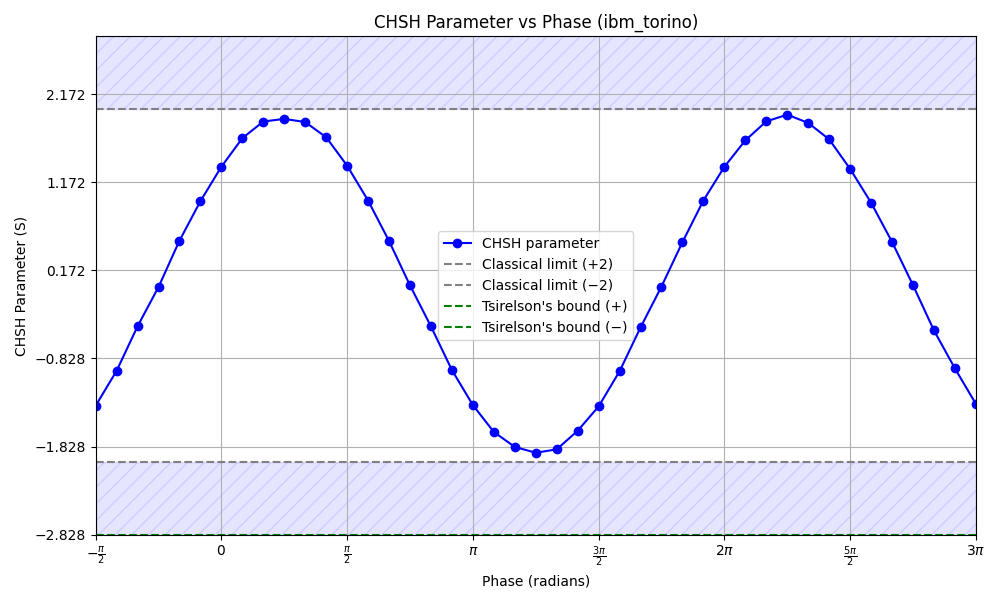
\includegraphics[width=1.0\textwidth]{figs/torino_anamoly.png}
    \caption{}
    \label{fig:torino}
\end{figure}

\section{Discussion}
The results were slightly unexpected because usually, if the qubit distance is getting longer, it means a deeper circuit is required to entangle the two qubits. This means that, in theory, more errors can occur. This implies that the $\max(|S|)$ should be lower. Interestingly, even though  \verb|ibm_torino| uses a newer processor, it has more two-qubit errors than the other two smaller backends. Overall, \verb|ibm_sherbrooke| performed the best. We assume that this is not because of the number of repetitions or \verb|SHOTS|, because we used 10000, which means that these results must have been very consistent for them to change the maximum value in an unexpected way. The biggest outlier is the `\verb|ibm_torino| maximum $S$ value at $2$ qubits, since this is the base circuit, and yet it performs the worst on it.

\section{Conclusions}

The popularization of the CHSH inequality in the late 1900s and early 21st century gave way to many novel experiments, which further enhanced human understanding of quantum physics. Using coding to model the behavior of particles in a quantum space allowed us to make conclusions on how and when particles are in an entangled state. Two variables, Alice and Bob, measure qubits simultaneously and apply gates that effectively increase the value of the CHSH parameter. We measured the qubits in 43 different phases between $[-\frac\pi2, 3\pi]$. After plotting the results on an x-y coordinate graph, there is an evident sinusoidal pattern that tells us at which intervals the CHSH inequality is being invalidated. When the phase was between 0 and 2, the plot points crossed the dotted line at y=2. This means that the S parameter of the CHSH inequality invalidates the rule that S must be less than or equal to 2. Additionally, this pattern occurs in periods of , which helps us understand at which sequences the two particles are entangled. 

Furthermore, we used the Qiskit library to create noise models, \verb|ibm_brisbane|, \verb|ibm_torino|, and \verb|ibm_sherbrooke|, to test the strength of entanglement of particles. We tested the particles at various distances. However, our data suggested that as the distance between the particles increased, the CHSH parameter also increased. This does not make logical sense because the strength of entanglement should theoretically decrease over increasing distance intervals, since the CNOT creating entanglement across qubits would be susceptible to more noise. In our case, the adverse effects of noise seemed to create high-quality entanglement, perhaps coincidentally. 



\newpage
\bibliography{refs}


\end{document}
